\newpage
\subsection{Tìm kiếm public key}

\subsubsection*{Mục tiêu}
Chức năng này cho phép người dùng tìm kiếm trong danh sách các public key đã lưu (của các liên hệ khác). Việc quản lý và tìm nhanh public key giúp người dùng dễ dàng sử dụng trong quá trình mã hóa, xác minh chữ ký, và chia sẻ an toàn.

\subsubsection*{Giao diện}
Giao diện tại tab \texttt{Owned Public Keys} trong dashboard bao gồm:
\begin{itemize}
    \item Bảng hiển thị danh sách các public key đã lưu: tên người gửi, email, timestamp và public key.
    \item Ô tìm kiếm theo email hoặc public key (tìm mờ, không phân biệt hoa thường).
    \item Dữ liệu được lấy động từ API \texttt{/owned\_keys}.
\end{itemize}

\begin{figure}[H]
    \centering
    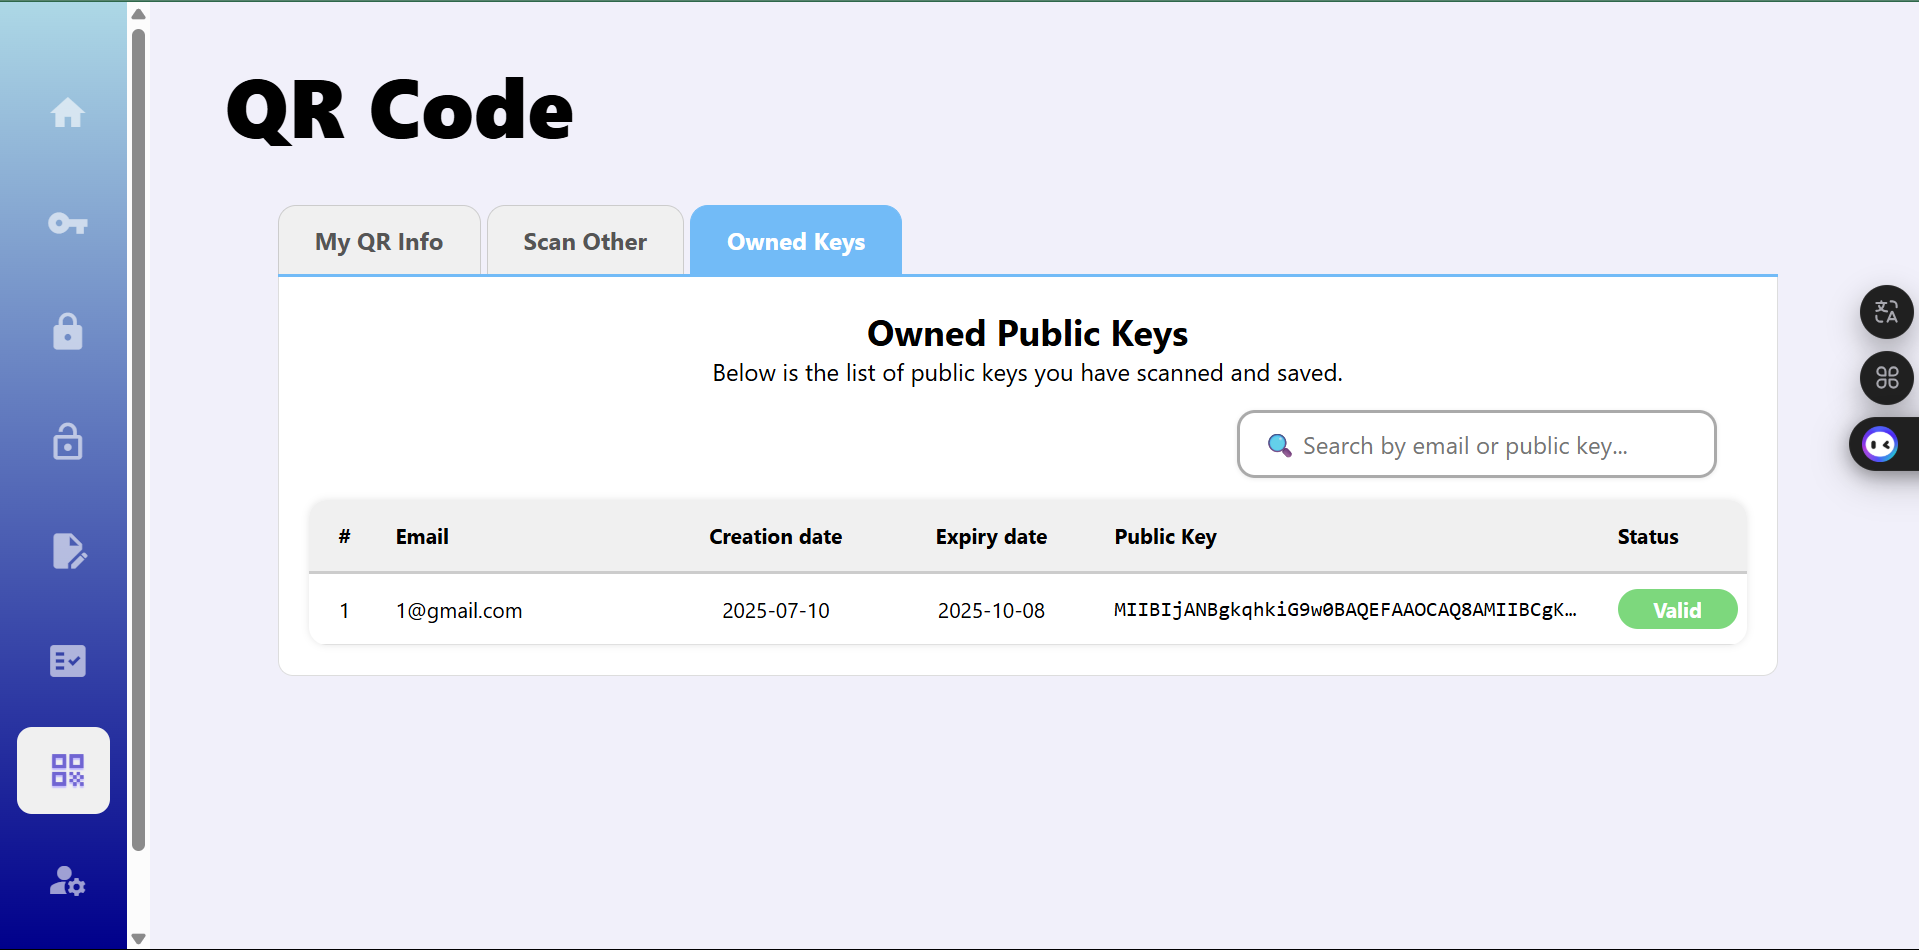
\includegraphics[width=0.85\textwidth]{img/14_pubkey/14_pubkey_ui.png}
    \caption{Danh sách contact - public key đã lưu}
\end{figure}

\subsubsection*{Quy trình thực hiện}
\begin{description}
    \item[\textbf{1. Truy cập tab Owned Keys}]
    Người dùng đăng nhập và truy cập trang dashboard → phần "Owned Public Keys" sẽ gửi request GET đến API \texttt{/owned\_keys}.

    \item[\textbf{2. API lấy dữ liệu}]
    Flask route \texttt{/owned\_keys} thực hiện:
    \begin{itemize}
        \item Kiểm tra phiên đăng nhập.
        \item Đọc file \texttt{contact\_public\_key.json} theo thư mục cá nhân người dùng.
        \item Chuyển danh sách public key về dạng JSON và trả về frontend.
    \end{itemize}

    \item[\textbf{3. Hiển thị và tìm kiếm}]
    \begin{itemize}
        \item JavaScript tạo bảng dữ liệu từ kết quả JSON trả về.
        \item Khi người dùng gõ từ khóa vào ô tìm kiếm, hàm \texttt{filterPublicKeys()} lọc các hàng phù hợp theo email hoặc chuỗi public key.
    \end{itemize}
\end{description}

\subsubsection*{Chi tiết kỹ thuật và thư viện bảo mật}
\begin{description}

    \item[\textbf{1. Cấu trúc lưu public key}]
    \begin{itemize}
        \item Mỗi người dùng có một file riêng: \texttt{<user\_email>/contact\_public\_key.json}
        \item Dạng JSON: \texttt{\{"abc@example.com": \{"name": ..., "public\_key\_pem": ...\}\}}
    \end{itemize}

    \item[\textbf{2. API trả dữ liệu public key}]
    \texttt{/owned\_keys} là route GET:
    \begin{itemize}
        \item Nếu chưa đăng nhập → trả lỗi \texttt{401 Unauthorized}.
        \item Nếu file danh bạ không tồn tại → trả danh sách rỗng.
        \item Ghi log trạng thái truy vấn bằng \texttt{log\_user\_action(...)} với số lượng public key tìm được.
    \end{itemize}

    \item[\textbf{3. Tìm kiếm phía client}]
    \begin{itemize}
        \item Hàm \texttt{filterPublicKeys()} lọc dữ liệu theo từ khóa không phân biệt hoa thường.
        \item Kiểm tra xem từ khóa xuất hiện trong email hoặc chuỗi public key PEM.
        \item Lọc trực tiếp trên DOM → không gọi lại API khi tìm kiếm.
    \end{itemize}

    \item[\textbf{4. Hiển thị QR code public key}]
    Hệ thống hỗ trợ hiển thị mã QR của public key khi người dùng click vào một contact cụ thể trong bảng danh sách. Điều này giúp việc chia sẻ public key giữa người dùng dễ dàng và nhanh chóng hơn (qua quét mã bằng điện thoại, Google Authenticator,...).

    \begin{itemize}
        \item Giao diện sử dụng sự kiện \texttt{onClick} hoặc nút \texttt{View QR} gắn với mỗi hàng trong bảng.
        \item Khi người dùng bấm chọn, mã public key PEM tương ứng sẽ được gửi đến route \texttt{/utils/generate\_qr} (hoặc sinh trực tiếp frontend).
        \item QR code được sinh từ chuỗi PEM hoặc JSON chứa các thông tin liên hệ và khóa công khai.
        \item Kết quả được hiển thị trong một modal hoặc khung bên cạnh dòng đã chọn.
        \item Mã QR cho phép người khác dễ dàng quét để lưu lại public key → hỗ trợ xác thực và mã hóa an toàn.
    \end{itemize}

    \begin{figure}[H]
        \centering
        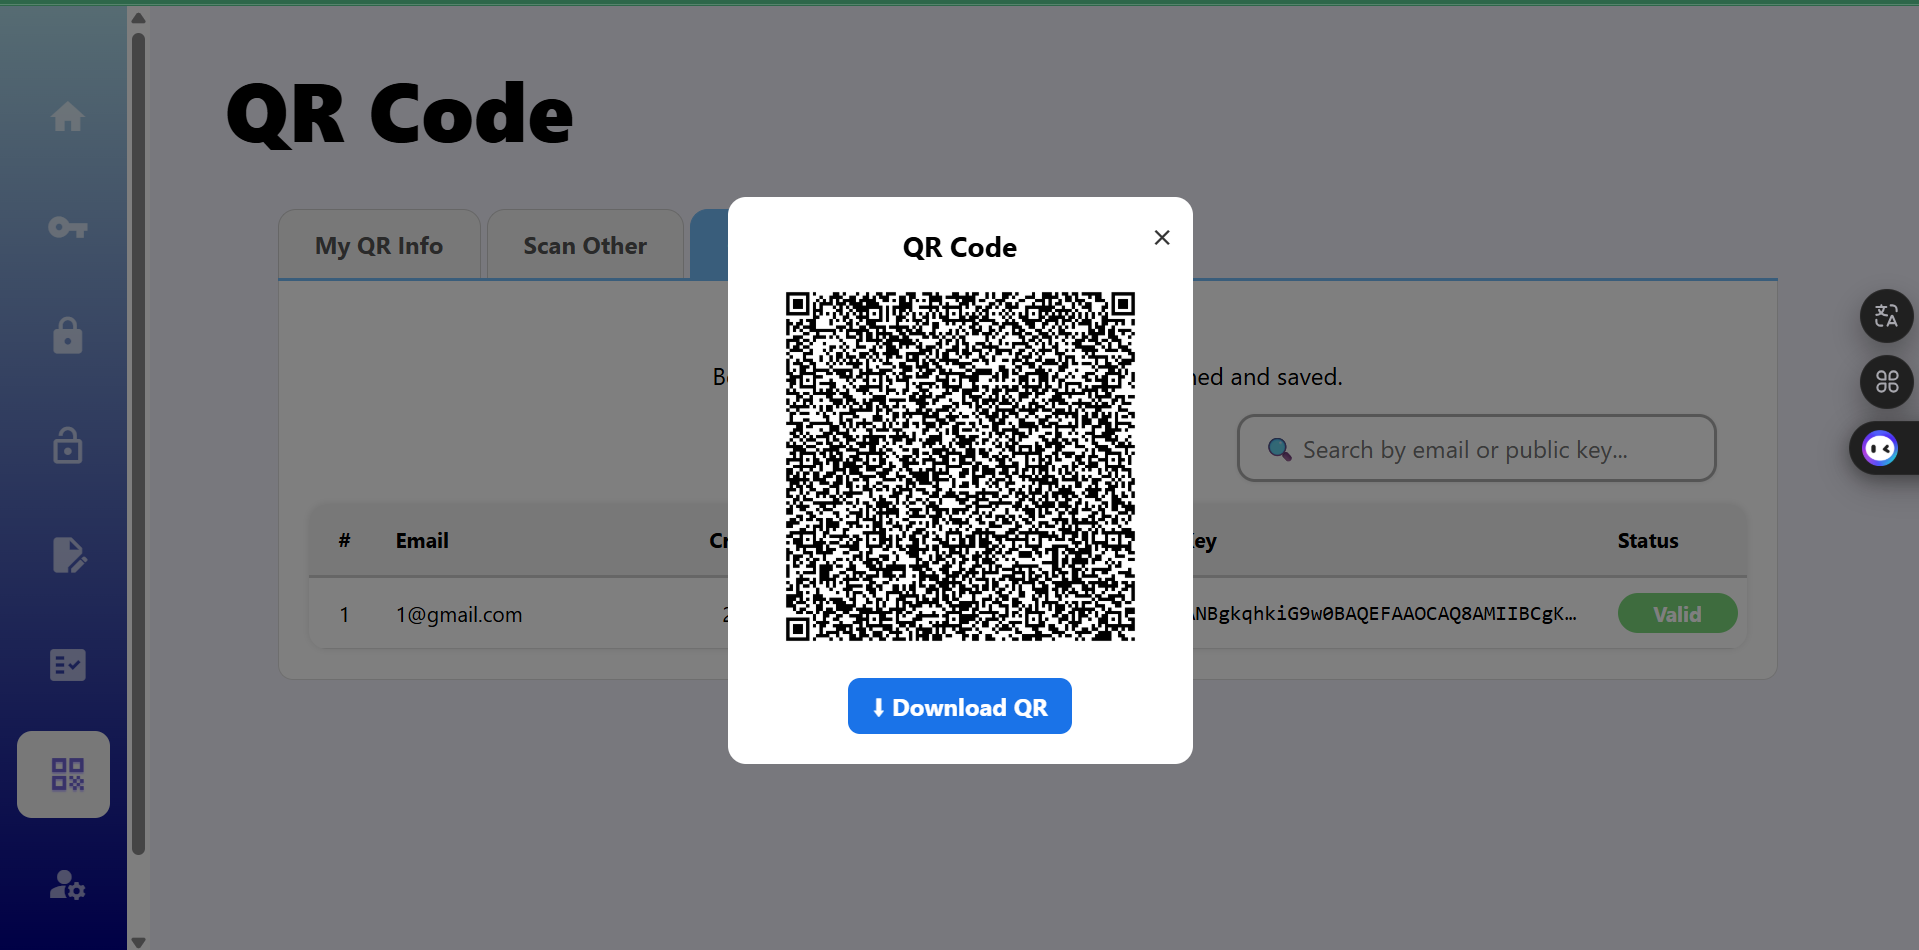
\includegraphics[width=0.85\textwidth]{img/14_pubkey/14_pubkey_qr.png}
        \caption{Pop-up QR của contact đã lưu}
    \end{figure}

    \item[\textbf{5. Bảo mật truy cập}]
    Chỉ người dùng đã đăng nhập mới được phép truy vấn danh sách public key đã lưu.
    \begin{itemize}
        \item File JSON được lưu riêng trong thư mục người dùng → cô lập dữ liệu từng tài khoản.
    \end{itemize}

\end{description}
